\section{Datenbank}
Die Datenbank wird durch eine MySQL Datenbank umgesetzt. Hierbei werden zu speichernde Dateien lediglich als Pfad in die Datenbank eingetragen. Die eigentlichen Daten sind auf dem Server angelegt.
\subsection{Datenbankaufbau}
\begin{figure}[h]
	\centering
	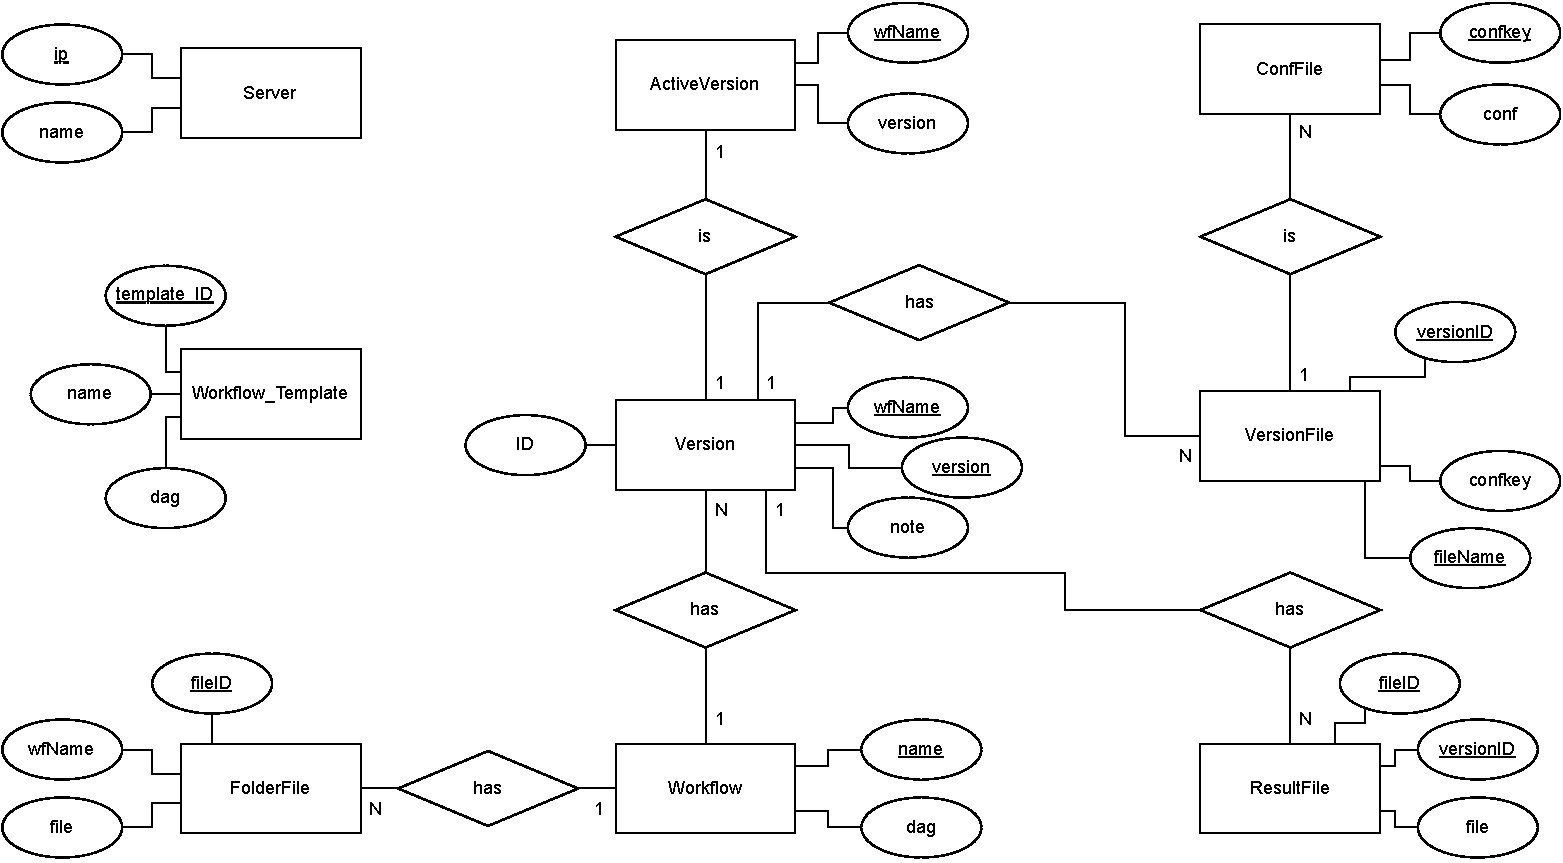
\includegraphics[width=0.85\textwidth]{res/er_diagram.pdf} 
	\caption{ER-Diagramm der Datenbank}
	\label{fig:er_diagram}
\end{figure}
Aus dem Entity Relationship Diagramm in Abbildung \ref{fig:er_diagram} folgt, dass die folgende Tabellen in der Datenbank anliegen

\paragraph{}
\begin{dataTable}
	\hline
	\textbf{Server} & & \\
	\hline
	ip & varchar(50) & $key$ \\
	\hline
	name & varchar(255) & $key$ \\
	\hline
\end{dataTable}

\paragraph{}
\begin{dataTable}
	\hline
	\textbf{WorkflowTemplate} &  & \\
	\hline
	template\textunderscore ID & int & $key; Auto\textunderscore Increment$\\
	\hline
	name & varchar(255) & $notNull$ \\
	\hline
	dag & varchar(255) & $notNull$\\
	\hline
\end{dataTable}

\paragraph{}
\begin{dataTable}
	\hline
	\textbf{Workflow} &  & \\
	\hline
	name & varchar(255) & $key$ \\
	\hline
	dag & varchar(255) & $notNull$\\
	\hline
\end{dataTable}

\paragraph{}
\begin{dataTable}
	\hline
	\textbf{FolderFile} &  & \\
	\hline
	filesID & int & $key; Auto\textunderscore Increment$ \\
	\hline
	wfname & varchar(255) & $notNull;$ name from Workflow\\
	\hline
	file & varchar(255) & $notNull$\\
	\hline
\end{dataTable}

\paragraph{}
\begin{dataTable}
	\hline
	\textbf{Version} & & \\
	\hline
	ID & int & $key; Auto\textunderscore Increment$ \\
	\hline
	wfName & varchar(255) & name from Workflow\\
	\hline
	version & varchar(127) & $notNull$ \\
	\hline
	note & varchar(1000) & \\
	\hline
\end{dataTable}

\paragraph{}
\begin{dataTable}
	\hline
	\textbf{ActiveVersion} & & \\
	\hline
	wfName & varchar(255) & $key;$ name from Workflow\\
	\hline
	version & varchar(127) &  from Version\\
	\hline
\end{dataTable}

\paragraph{}
\begin{dataTable}
	\hline
	\textbf{VersionFile} & & \\
	\hline
	versionID & int & $key;$ ID from Version \\
	\hline
	filename & varchar(255) & $key$\\
	\hline
	confKey & int & $notNull;$ from ConfFiles \\
	\hline
\end{dataTable}

\paragraph{}
\begin{dataTable}
	\hline
	\textbf{ConfFile} & & \\
	\hline
	confKey & int & $key; Auto\textunderscore Increment$ \\
	\hline
	file & varchar(255) & $notNull$ \\
	\hline
\end{dataTable}

\paragraph{}
\begin{dataTable}
	\hline
	\textbf{ResultFile} &  & \\
	\hline
	versionID & int & $key;$ ID from Version \\
	\hline
	filesID & int & $key; Auto\textunderscore Increment$ \\
	\hline
	file & varchar(255) & $notNull$\\
	\hline
\end{dataTable}

\paragraph{Anmerkung} Die dag Datei hätte als Schlüssel zwischen Workflow\_Template und Workflow fungieren können, ist aber redundant für alle Operationen auf einem Workflow.
Deshalb wurde entschieden die Datei bei einer Workflowerstellung direkt zu kopieren.


\newpage